\documentclass[runningheads,parskip=full]{scrreprt}
%
\usepackage{makeidx}  % allows for indexgeneration
\usepackage[pdftex]{hyperref}
\usepackage{graphicx}
\usepackage{url}
\usepackage{amsmath}
\usepackage{gensymb}
\usepackage[all]{nowidow}
\usepackage{multirow}

%

\newenvironment{packed_enum}{
\begin{enumerate}
  \setlength{\itemsep}{1pt}
  \setlength{\parskip}{0pt}
  \setlength{\parsep}{0pt}
}{\end{enumerate}}

\newenvironment{packed_item}{
\begin{itemize}
  \setlength{\itemsep}{1pt}
  \setlength{\parskip}{0pt}
  \setlength{\parsep}{0pt}
}{\end{itemize}}


\def\wl{\par \vspace{\baselineskip}}

\begin{document}

\pagestyle{headings}  % switches on printing of running  heads

\title{
Energy Efficient Considerations for HPC Procurement Documents \\
\bigskip
\normalsize{(version 0.45)}
}

\author{The Energy Efficient High Performance Computing Working Group}


\date{ }
\maketitle              % typeset the title of the contribution

\tableofcontents
\listoftables
\listoffigures

%
\chapter{Introduction}
This document captures some best practices to consider when writing procurement documents for supercomputer acquisitions. These best practices concern energy efficiency, especially capabilities to measure and manage both power and energy consumption. The document draws upon recent procurement documents created and used by two major supercomputing sites. In addition the document modifies and supplements the material from these procurement documents with input from experts in energy efficient HPC.
 
The team that wrote this draft consists exclusively of members from the user community, mostly from US DOE Labs.  General publiction will include review and feedback from vendors.

Although  progress has been made, there remains much room for improvement in HPC energy efficiency. This document sets this year’s vision (2013) for systems to be delivered and accepted in two years (2015). It identifies priorities and sets an immediate goal.  Becasue it is expected that these priorities will change and that the bar will rise over time, this document will be refreshed on a yearly basis.

Some of the content below is informational and as such is intended to set the context for the acquisition, but not to be used as a requirement.  Additional content reflects requirements and is intended to specify system features and capabilities.  These requirements are categorized as mandatory, important, or enhancing.

The intent is that this document encourage dialogue about priorities and requirements for HPC system energy efficient features and capabilities while recognizing that each HPC center has its own unique mission with differing priorities. The requirements discussed here are intended to draw lines in the sand that can be easily re-drawn, not to build isolating fences.
 
Finally, this document is intended to be high level while remaining vendor and technology neutral.  It should encourage innovation and not pick a particular vendor or solution.

The content is organized into five categories, all focused on energy efficiency.  

Measurement, benchmarks and management focus almost exclusively on system hardware and system software, but also span applications.  

The other two categories are general objectives and cooling.  These two areas span infrastructure and the supercomputer system itself (mostly system hardware, but some aspects of system software as well).

Conventions:

Information: info

\begin{packed_enum}
\item
enhancing
\item
important
\item
mandatory
\end{packed_enum}
\label{sec:intro}

\chapter{Measurements}
\begin{itemize}
\item[{\textbf{(info)}}]
Power and energy measurement capabilities are necessary to meet the needs of future 
supercomputing power and energy constraints. These mechanisms may differ in implementation 
and purpose, and include capabilities for measuring the energy consumption of entire systems, 
platforms (subsystems), cabinets, nodes and components.  

\item[{info}]
This section is primarily focused on measuring the system power and energy, which includes system hardware and software.  

\item[{mandatory}]
The vendor shall provide the mechanism, interface, hardware, firmware, software, and any other elements that are necessary to capture the individual power and energy measurements. 

\item[{mandatory}]
This capability should have no (or minimal and defined) impact on the computation, security, and energy consumption of the equipment.  The vendor must describe the impact, preferably in quantitative terms.  

\item[{mandatory}]
Scalable tools to extract accumulate and display power, energy and temperature information (accumulated energy and peak, instantaneous as well as average power between any two points in time) should be delivered.

\item[{mandatory}]
The power and energy data must be exportable with at least a comma separated value or a user-accessible API. 

\item[{mandatory}]
For power, energy (and discrete current and voltage measurements if available) a detailed description of the measurement capabilities must be provided, including a specified value for measurement precision, accuracy and how data samples are time-stamped. WE HAD A LOT OF DISCUSSION ABOUT PRECISION and ACCURACY, SHOULD WE EXPAND ON WHAT WE WANT HERE FOR THE ENTIRE DOCUMENT? CAN WE PROVIDE A SPECIFIC REQUIREMENT OR BE MORE DESCRIPTIVE ABOUT WHAT WE WANT HERE – JHL? Reference ANSI C12.1

\item[{info}]
Why hierarchy?

	The document is formatted in somewhat of a hierarchical fashion. The purpose of this is to address the various current and anticipated future use cases related to this topic. Component level measurement, for example, is required for fine-grained application power and energy analysis; likewise, component level control could be used to shift power from one component to another based on specific application requirements. Measurement at node level granularity is necessary for understanding the power and energy characteristics of a multi-node application, for example. While cabinet level measurement might have fewer current use cases, cabinet level power capping, as well as node level, are emerging as important requirements in recent procurements. Platform level measurement and control has many facility inspired use cases and is a critical piece of overall platform management.

\item[{info}]
Reported Values verses Internal Samples

%INCLUDE FIG 3-1 
\begin{figure}[htbp]
\centering
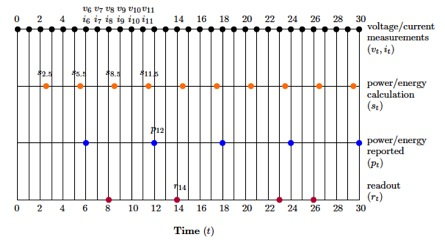
\includegraphics[width=4in]{fig1}
\caption{Power Profile HPL Run}
\label{fig:powprof}
\end{figure}

A number of terms are used in this document to describe measurement capabilities. It is important to understand the context in which the terms are used. Figure~\ref{fig:powprof} illustrates these terms. The x-axis of Figure~\ref{fig:powprof} is Time (in generic units). Note, Figure~\ref{fig:powprof} represents a range of possible capabilities that are useful for this discussion, it does not imply that these specific capabilities are a requirement.

\begin{itemize}
\item
The top horizontal line represents points in time when discrete internal current and voltage measurements are sampled at the device level. These samples are not necessarily exposed externally. At each time interval a voltage and current sample is internally measured (v6, i6 pair for example).  
\item
The second line down represents the points in time when an internal power and/or energy calculation is performed. Again, the result is not necessarily exposed externally.
\item
The third line down represents the points in time a reported value is available to be read, externally. Each reported value could represent an average power, an instantaneous power, or an accumulated energy value, depending on the device capabilities. For example, point P12 could simply be the power value calculated at S8.5 or S11.5. P12 could also be the average power of points S8.5 and S11.5, or all of the calculated power samples prior to P12. P12 could likewise be an accumulated energy value representing any range of power samples up to that point in time. The important distinction is the difference between the device’s internal sampling capability (frequency of and what the samples represent) and the external reported value capability of the device (again, frequency of and what the values represent).
\item
Finally, the forth line down represents when the user actually obtains the reported value readout. It is critical that the timestamp of the reported value represents the time, as accurately as possible, of the measurement. Notice that the actual readout takes place at various time intervals following the availability of the reported value. This emphasizes the importance of time stamping at the time of measurement, not at the time of reading the value.
\end{itemize}

For example, a measurement device may be capable of producing 100 discrete power samples per second (internally). The power calculation (sample) and availability of the reported value of this same device may be equivalent to the lowest level sampling frequency, but no greater. Both, are typically less than the internal sampling frequency. For example, the same device may have the ability of producing a reported a value at 10 times per second. This reported value could be a power value averaged over 10 seconds, an accumulated energy value that includes 10 additional seconds with each new reported value, or simply a discrete (instantaneous) power value for that moment in time. 

Generally speaking, the requirements for the frequency of the reported value depend on what the reported value represents. If the reported value is a discrete power value then a higher frequency of reported value is typically desired. If the reported value represents an average power or accumulated energy value, reported frequency is less important than the internal sampling frequency that is used to derive the reported average power or energy value.
\end{itemize}

\section{System, Platform, and Cabinet Level Measurements}

%INSERT TABLE 1
\begin{table}[htbp]
\caption{System, platform, and cabinet requirements for internal and reported frequency}
\label{tab:spclevel}
\begin{tabular}{|p{3.0cm}|p{3.5cm}|p{3.5cm}|p{3.5cm}|} \hline
& & \textbf{Internal Sample}&\textbf{External}\\ 
& & \textbf{Frequency}&\textbf{Reported Value}\\ 
& & & \textbf{Frequency}\\ \hline

\textbf{Mandatory} &
Discrete power (W)&
\mbox{$ \ge $} 1 per second &
\mbox{$ \ge $} 1 per second \\

& 
Average Power (W) &
\mbox{$ \ge $} 10 per second &
\mbox{$ \ge $} 1 per second \\

& 
Energy (J) &
\mbox{$ \ge $} 10 per second &
\mbox{$ \ge $} 1 per second \\ \hline

\textbf{Important} & 
Discrete power (W)&
\mbox{$ \ge $} 10 per second &
\mbox{$ \ge $} 10 per second \\

& 
Average Power (W) &
\mbox{$ \ge $} 100 per second &
\mbox{$ \ge $} 1 per second \\

& 
Energy (J) &
\mbox{$ \ge $} 100 per second &
\mbox{$ \ge $} 1 per second \\ \hline 

\textbf{Enhancing} & 
Discrete power (W)&
\mbox{$ \ge $} 100 per second &
\mbox{$ \ge $} 1000 per second \\

& 
Average Power (W) &
\mbox{$ \ge $} 1000 per second &
\mbox{$ \ge $} 1 per second \\

& 
Energy (J) &
\mbox{$ \ge $} 1000 per second &
\mbox{$ \ge $} 10 per second \\ \hline

\end{tabular}
\end{table}
\begin{itemize}
\item[(info)]
The system level may vary by site and architecture, but could be so broad as to include all of the parts of the system that explicitly participate in performing any workload(s). This might include supporting internal and external power and cooling equipment as well as internal and external communication and storage sub-systems. 
\item[(info)]
The platform is distinguished from the system so as to differentiate compute from other system-level equipment (such as external storage) that may be managed distinctly, but together comprise a system. 
\item[(info)]
The cabinet (or rack) is the first order discretization of the platform level measurement. The cabinet may be part of the compute, storage or networking platform. 
\item[(mandatory)]
Must be able to measure system, platform, and cabinet power and energy.

	Table~\ref{tab:spclevel} lists the mandatory, important and enhancing requirements for the internal sampling frequency (internal device capability) and the external reported value frequency (data available to the consumer) at the system, platform and cabinet level. Figure 1 should be referenced in conjunction with Table 1 to help clarify these requirements. Note that Figure 1 also depicts readout, i.e. when the consumer chooses to read the data. Readout rate will not be addressed in the requirements since readout rate is driven by the computer and limited by the reported value frequency. The details describing the internal sampling frequency (voltage and current or power), how the average power and/or energy value is calculated \textbf{must} be provided.

\item[(mandatory)]
The power and energy values must be based on electrical measurements (e.g. based on shunts or hall effect sensors). Values that are derived from heuristic models based on architectural events or system state (e.g. RAPL) can complement but not replace them.

\item[(important)]
The vendor shall assist in the effort to collect these data in whatever other subsystems are provided (e.g., another vendor’s back-end storage system). 

\item[(important)]
Those elements of the system, platform and cabinet that perform infrastructure-type functions (e.g., cooling and power distribution), must be measured separately with the ability to isolate their contribution to the power and energy measurements.  

\end{itemize}

\section{Node Level Measurements}

%INSERT TABLE 2
\begin{table}[htbp]
\caption{Node Level Requirements for internal and reported frequency}
\label{tab:nodelevel}
\begin{tabular}{|p{3.0cm}|p{3.5cm}|p{3.5cm}|p{3.5cm}|} \hline
& & \textbf{Internal Sample}&\textbf{External}\\ 
& & \textbf{Frequency}&\textbf{Reported Value}\\ 
& & & \textbf{Frequency}\\ \hline

\textbf{Mandatory} &
Discrete power (W)&
\mbox{$ \ge $} 1 per second &
\mbox{$ \ge $} 1 per second \\

& 
Average Power (W) &
\mbox{$ \ge $} 10 per second &
\mbox{$ \ge $} 1 per second \\

& 
Energy (J) &
\mbox{$ \ge $} 10 per second &
\mbox{$ \ge $} 1 per second \\ \hline

\textbf{Important} & 
Discrete power (W)&
\mbox{$ \ge $} 10 per second &
\mbox{$ \ge $} 10 per second \\

& 
Average Power (W) &
\mbox{$ \ge $} 100 per second &
\mbox{$ \ge $} 1 per second \\

& 
Energy (J) &
\mbox{$ \ge $} 100 per second &
\mbox{$ \ge $} 1 per second \\ \hline 

\textbf{Enhancing} & 
Discrete power (W)&
\mbox{$ \ge $} 100 per second &
\mbox{$ \ge $} 1000 per second \\

& 
Average Power (W) &
\mbox{$ \ge $} 1000 per second &
\mbox{$ \ge $} 1 per second \\

& 
Energy (J) &
\mbox{$ \le $} 1000 per second &
\mbox{$ \le $} 10 per second \\ \hline

\end{tabular}
\end{table}

\begin{itemize}

\item[(info)]
A node level measurement shall consist of the combined measurement of all components that make up a node for the architecture. For example, components may include the CPU, memory and the network interface. If the node contains other components such as spinning or solid state disks they shall also be included in this combined measurement. The utility of the node level measurement is to facilitate measurement of the power and energy characteristics of a single application. The node may be part of the network or storage equipment, such as network switches, disk shelves and disk controllers.   

\item[(important)]
The ability to measure the power and energy of any and all nodes must/should be provided.  NOTE: Should this be mandatory? Change must/should appropriately.

	Table~\ref{tab:nodelevel} lists the mandatory, important and enhancing requirements for the internal sampling frequency (internal device capability) and the external reported value frequency (data available to the consumer) at the node level. Figure 1 should be referenced in conjunction with Table 1 to help clarify these requirements. Note that Figure 1 also depicts readout, i.e. when the consumer chooses to read the data. Readout rate will not be addressed in the requirements since readout rate is driven by the computer and limited by the reported value frequency. The details describing the internal sampling frequency (voltage and current or power), how the average power and/or energy value is calculated must be provided.

\item[(mandatory)]
The power and energy values must be based on electrical measurements (e.g. based on shunts or hall effect sensors). Values that are derived from heuristic models based on architectural events or system state (e.g. RAPL) can complement but not replace them.
\end{itemize}


\section{Component Level Measurement}

%INSERT TABLE 3
\begin{table}[htbp]
\caption{Component Level Requirements for internal and reported frequency}
\label{tab:comlevel}
\begin{tabular}{|p{3.0cm}|p{3.5cm}|p{3.5cm}|p{3.5cm}|} \hline
& & \textbf{Internal Sample}&\textbf{External}\\ 
& & \textbf{Frequency}&\textbf{Reported Value}\\ 
& & & \textbf{Frequency}\\ \hline

\textbf{Mandatory} &
Discrete power (W)&
\mbox{$ \ge $} 1 per second &
\mbox{$ \ge $} 1 per second \\

& 
Average Power (W) &
\mbox{$ \ge $} 10 per second &
\mbox{$ \ge $} 1 per second \\

& 
Energy (J) &
\mbox{$ \ge $} 10 per second &
\mbox{$ \ge $} 1 per second \\ \hline

\textbf{Important} & 
Discrete power (W)&
\mbox{$ \ge $} 10 per second &
\mbox{$ \ge $} 10 per second \\

& 
Average Power (W) &
\mbox{$ \ge $} 100 per second &
\mbox{$ \ge $} 1 per second \\

& 
Energy (J) &
\mbox{$ \ge $} 100 per second &
\mbox{$ \ge $} 1 per second \\ \hline 

\textbf{Enhancing} & 
Discrete power (W)&
\mbox{$ \ge $} 100 per second &
\mbox{$ \ge $} 1000 per second \\

& 
Average Power (W) &
\mbox{$ \ge $} 1000 per second &
\mbox{$ \ge $} 1 per second \\

& 
Energy (J) &
\mbox{$ \le $} 1000 per second &
\mbox{$ \le $} 10 per second \\ \hline

\end{tabular}
\end{table}
\begin{itemize}

\item[(info)]
Components are the physically discrete units that comprise the node. This level of measurement is important to analyze application energy/performance trade-offs. This level is analogous to performance counters and carries many of the same motivations.  Components may not only be silicon devices.  For example, it would be useful to know how much fan energy is being used by the Muffin fans at the back of the rack or by some active rear door cooling methodology.  Also, some systems may have a CDU.  How much energy is being used by the CDU for motors, fans.
	
\item[(enhancing)]
The ability to measure the power and energy of each individual component must (or should if this is enhancing?) be provided.
	
	Table~\ref{tab:comlevel}  lists the mandatory, important and enhancing requirements for the internal sampling frequency (internal device capability) and the external reported value frequency (data available to the consumer) at the node level. Figure 1 should be referenced in conjunction with Table 1 to help clarify these requirements. Note that Figure 1 also depicts readout, i.e. when the consumer chooses to read the data. Readout rate will not be addressed in the requirements since readout rate is driven by the computer and limited by the reported value frequency. The details describing the internal sampling frequency (voltage and current or power), how the average power and/or energy value is calculated \textbf{must} be provided.

\item[(mandatory)]
The power and energy values must be based on electrical measurements (e.g. based on shunts or hall effect sensors). Values that are derived from heuristic models based on architectural events or system state (e.g. RAPL) can complement but not replace them.
\end{itemize}




\label{sec:measurements}

\chapter{Management and Control}
\begin{itemize}
\item[\textbf{(info)}]
As with the measurement capabilities described above, power and energy management and control 
capabilities (hardware and software tools and application programming interfaces (APIs)) are 
necessary to meet the needs of future supercomputing energy and power constraints. It is 
extremely important that [Customer] utilize early capabilities in this area and start 
defining and developing advanced capabilities and integrating them into a user friendly, 
production environment.  

The vendor shall provide mechanisms to manage and control the power and energy 
consumption of the system. These mechanisms may differ in implementation and purpose.  
Below are envisioned usage models for these management capabilities.  They are categorized 
loosely by where the management occurs. It is envisioned that this capability will evolve 
over time from initial monitoring and reporting capabilities, to management (including 
activities like 6-sigma continuous improvement), and even to autonomic controls.   

These usage models are not requirements for the vendor, but rather suggestive 
examples that serve to help clarify the requirements for measurement capabilities 
described in Section~\ref{sec:measurements} above. Furthermore, it is recognized that 
many of these solutions would be provided by a third party, not by the system vendor.  
\end{itemize}

\section{Datacenter/Infrastructure}
\begin{itemize}
\item[\textbf{(info)}]
Respond to utility requests or rate structures. For example, cut back usage 
during high load times, limit power during expensive utility rate times of the day. 

 ``Power capping'' the system allows for provisioning the infrastructure for closer 
to average usage, leading to substantial infrastructure savings compared to those 
centers which are designed for theoretical peak usage.  

Respond to demand requests, including increases in load to accommodate waste 
heat recovery, renewable energy, etc.

Manage rate of power changes; e.g., avoid spikes.  As another example, the large variations of 
harmonic current produced by computer loads may need to be balanced in the datacenter as well 
as the site's broader infrastructure and even the grid.  
\end{itemize}

\section{System Hardware and Software}
\begin{itemize}
\item[\textbf{(info)}]
Reduce power utilization during ``design days'' so as to enable use of free cooling 
without backup chillers.  Implement alarm and/or automatic shut-down that responds to environmental 
temperature excursions that are outside of the facility design envelope by reducing system loads.  

Identify higher than normal power draw components needing maintenance and/or replacement.   
posibly also identify higher than normal power draw usage from SW- perhaps 
that is ``stuck'' in an infinite loop-back mode.     

Proliferate power scaling and management beyond computation, to memory, communication, 
I/O and storage.  For example, consider under and overclocking and OS/hardware control of the 
total amount of energy consumed 

In addition to traditionally compiling for performance, the compiler vendor may want 
to provide the user with mechanisms to compile for energy efficiency. The possible mechanisms 
may include the following.

\begin{itemize}
\item
Compiler flags for specifying performance-energy trade-offs or regarding energy efficiency 
as an optimization goal or a constraint.
\item
Programming directives for conveying user-level information to the compiler for 
better optimization in the context of energy efficiency.
\item
Program constructs to promote energy as the first-class object so that it can be 
manipulated directly in source code.
\item
Compiler-based tools for reporting analyzed results regarding the energy efficiency of applications.     
\end{itemize}
\end{itemize}

\section{Applications, Algorithms, Libraries}
\begin{itemize}
\item[\textbf{(info)}]
Provides programming environment support that leads to enhanced energy efficiency.

Reduce wait-states. Examples are the following:

\begin{itemize}
\item
Schedule background I/O activity more efficiently with I/O interface extensions 
to mark computation and communication dominant phases. 
\item
Use an energy-aware MPI library which is able to use information of wait-states 
to reduce energy consumption.
\end{itemize}

Reduce the power draw in wait-states. An example is the following:

\begin{itemize}
\item
Attain energy reduction for task-parallel execution of dense and sparse linear algebra 
operations on multi-core and many-core processors, when idle periods are leveraged 
by promoting CPU cores to a power-saving C-state.
\end{itemize}

Scale resources appropriately. Examples are the following:
\begin{itemize}
\item
Apply the phase detection procedure to parallel electronic structure calculations, 
performed by a widely used package GAMESS. Distinguishing computation and communication 
processes have led to several insights into the role of process-core mapping in the 
application of dynamic frequency scaling during communications.
\item
Analyze the energy-saving potential by reducing the voltage and frequency of processes 
not lying on a critical path, i.e., those with wait-states before global synchronization points.
\item
Enabling network bandwidth tuning for performance and energy efficiency.
\end{itemize}

Select appropriate energy-performance trade-off. An example is the following:
\begin{itemize}
\item
Optimize the power profile of a dense linear algebra algorithm (PLASMA) by 
focusing on the specific energy requirements of the various factorization 
algorithms and their stages.
\end{itemize}

Programming and performance analysis tools. An example is the following.
\begin{itemize}
\item
Counters, accumulators, in-band support.
\end{itemize}

Open up control of these policies so that we can turn them on and off including   
zero setting if a policy is detrimental to our applications at scale. 
\end{itemize}

\section{Schedulers, Middleware, Management}
\begin{itemize}
\item[\textbf{(info)}]
Putting hardware into the lowest reasonable power state or switching off idle 
resources (nodes, storage, etc.) when job scheduling cannot allow for full utilization. 

Different power states. Careful about how we switch a power state off.  Cannot affect reliability.  
Sleep states are probably the best direction.  Response time is much better.

Energy-aware scheduling. Develop mechanism to automatically select processor 
frequency for which energy to solution is minimized for a specific application.

Demand response (as in the ability to react to electrical grid based incentives)
requires enhanced scheduling tools. 

Evolving hardware features will likely require enhanced system software and scheduling 
tools with control at all levels of the hierarchy, from the system down to the components.  
An example might be a scenario where you have a high priority job and there are available 
nodes to run the job; but if the job runs at the desired P-state, the system would exceed some 
notion of a power cap.  In this situation, can one dynamically alter the P-state of lower 
priority jobs to allow them to continue, perhaps at a slower rate, while also accommodating 
the new, high priority job.
\end{itemize}


\label{sec:management}

\chapter{Benchmarks}
\begin{itemize}

\item[(info)]
Since power and energy costs, both operational and capital, are increasingly significant, it is very important to understand the power and energy efficiency requirements of the system.  This is best understood when running workloads; either applications or benchmarks.  Each site will have to select the workloads to run as part of the procurement and acceptance process.  These workloads may differentially exercise or stress various sub-systems; compute (CPU, GPGPU, etc.), I/O, Networks (Internal, facility and WAN).  They may focus on applications that are based on integer as well as floating point computations.

\item[(mandatory)]
[Customer] shall specify the set of benchmarks they want. Vendors shall provide the power and energy efficiency requirements, and run times of a set of benchmarks. 

\item[(mandatory)]
The types of problem in the benchmarks shall cover compute problems, memory problems, networking problems, idle and sleep system state

\item[(info)]
Suggested examples: HPL (compute problem), Integer-dominant codes (compute problem), Graph500 (memory/networking problem), GUPS, GUPPIE,  mySQL and non-mySQL database applications, and systemBurn developed at ORNL. 

\item[(mandatory)]
Customers shall specify the run rules and the measurement quality. Each benchmark must be measurable using the Green500 run rules and attain a Level 2 measurement quality. 

\item[(important)]
Customers shall specify the run rules and the measurement quality. Each benchmark must be measurable using the Green500 run rules and attain a Level 3 measurement quality. 

\item[(important)]
Vendors shall work with Customers to provide the power and energy effiency requirements of a set of site-supplied workloads. These workloads will reflect the typical case, not the extremes so that vendors can design around the typical case. 

\item[(important)]
Customers may also require application power profiles with power and energy requirements.
\end{itemize}


\label{sec:benchmarks}

\chapter{General Objectives}
\begin{itemize}

\item[(info)]
The vendor shall provide [equipment, services and/or resources] that – among other objectives – establish a highly energy efficient solution at justifiable cost.  The proposed solutions should demonstrate net benefits under normal production conditions.  
\end{itemize}

\section{Energy-related Total Cost of Ownership (TCO)}

\begin{itemize}

\item[(enhancing)]
It is an objective of [Customer] to encourage innovative programs whereby the vendor and/or [Customer] are incentivized to reduce the costs for energy and/or power related capital expenditures as well as the operational costs for energy.  This may be for the system, data center and/or broader site.  By doing this, the vendor would be reducing the energy-related TCO for [Customer].  The vendor is encouraged to describe their support for these innovative programs in qualitative as well as quantitative terms.

\item[(info)]
An example of an innovative program for bringing the energy/power element of TCO to the front was used by LRZ.  Their procurement was based on TCO whereby the budget covered not just investment and maintenance, but operational costs as well. The intent was to provide a clear incentive for the vendor to deliver a solution that would yield low operational costs and, thereby, lower TCO.

\end{itemize}

\section{Power Usage Effectiveness (PUE)}

\begin{itemize}

\item[(info)]
It is an objective of [Customer] to run a highly energy efficient data center.  One measure for data center efficiency is PUE.  It is recognized that the metric PUE has limitations.  For example, solutions with cooling subsystems that are built into the computing systems will result in a more favorable PUE than those that rely on external cooling, but are not necessarily more energy efficient.  In spite of these limitations, PUE is a widely adopted metric that has helped to drive energy efficiency.

\item[(enhancing)]
The US Department of Energy Office of the Chief Information Officer has set a requirement to achieve an average PUE of 1.4 by 2015.  As a result, the vendor is encouraged to qualitatively describe their support for helping [Customer] to meet this requirement.

\end{itemize}

\section{Total Usage Effectiveness (TUE)}

\begin{itemize}

\item[(info)]
TUE is another metric that has been developed to overcome the limitations of the PUE metric.  Specifically, it resolves the issue of PUE differences due to infrastructure loads moving from inside to outside the box.  TUE is the total energy into the data center divided by the total energy to the computational components inside the IT equipment.

\item[(enhancing)]
The vendor is encouraged to qualitatively describe their support for measuring TUE.
\end{itemize}

\section{Energy Re-Use Effectiveness (ERE)}

\begin{itemize}

\item[(info)]
Some sites have the ability to utilize the heat generated by the data center for productive uses, such as heating office space.  Energy re-use is not strictly adding to the energy efficiency of either the computing system or the data center, but it can reduce the energy requirements for the surrounding environment.  For those sites, it would be an objective of [Customer] to achieve an ERE < 1.0.  

\item[(enhancing)]
The vendor is encouraged to qualitatively describe their support for helping [Customer] to achieve an ERE < 1.0.  

\end{itemize}

\section{Power Distribution}
\begin{itemize}
\item[(important)]
The vendor is encouraged to qualitatively describe energy efficient and innovative solutions that help to reduce conversion losses in the data center.
\end{itemize}


\label{sec:genobjectives}

\chapter{Cooling}
\section{Liquid Cooling}

\begin{itemize}
\item[\textbf{(info)}]
For systems designed to be liquid-cooled, there is an opportunity for large energy 
savings compared to air-cooled designs.  Since liquids have more heat capacity than 
air, smaller volumes can achieve the same level of cooling and can be transported 
with minimal energy use.  In addition, if heat can be removed through a fluid phase 
change, heat removal capacity is further increased.  By bringing the liquid closer 
to the heat source, effective cooling can be provided with higher temperature fluids.  
The higher temperature liquid cooling can be produced without the need for 
compressor-based cooling.

\item[\textbf{(info)}]
[Customer] will specify the type of liquid cooling systems contained within the datacenter.  
The range of liquid supply temperatures available in the center corresponding to 
ASHRAE-recommended classes (W1-W4) will be provided to the vendor.  

\item[\textbf{(info)}]
A traditional datacenter is cooled using compressor-based cooling (i.e., chillers or 
CRAC units) and additional heat rejection equipment such as cooling towers or dry coolers.  
These liquid-cooled systems operate within ASHRAE-recommended ranges W1 and W2.  Systems 
designed to operate in these ranges will have limited energy efficiency capability.

\item[\textbf{(important)}]
For improved energy efficiency and reduced capital expense, many datacenters can be 
operated without compressor-based cooling, by using cooling towers or dry coolers 
combined with water-side economizers. These datacenters can operate within the ASHRAE 
W3 range and accordingly, systems should be requested to operate in this range.

\item[\textbf{(enhancing)}]
In most locations, liquid cooling of up to 45\celsius~can be provided using dry coolers.  
The ASHRAE W4 classification was defined to accommodate this low energy form of cooling.  
For this type of infrastructure, ASHRAE W4 class should be requested.  

\item[\textbf{(info)}]
Parameters like pressure, flow rate, and water quality may also be specified by each site 
in its procurement documents.  ASHRAE provides guidance on these parameters, although 
they are not defined in this guideline. 
\end{itemize}
 
\section{Air Cooling}
\begin{itemize}
\item[\textbf{(info)}]
ASHRAE Thermal Guidelines (2011) define environmental classes that allow temperatures 
up to 40\celsius~and 45\celsius.  

Figure~\ref{fig:ITenviron} is a pschometric chart illustratiing these new environmental 
temperature and humidity limits along with the recommended limits.

\item[\textbf{(mandatory)}]
The system must be able to operate in a Class A1 environment.  

\item[\textbf{(important)}]
It is better to operate in a Class A2 environment (important) 

\item[\textbf{(enhancing)}]
All other things equal, it is best to operate in a Class A3 environment.
\end{itemize}

%INCLUDE FIG 5-1
\begin{figure}[htbp]
\centering
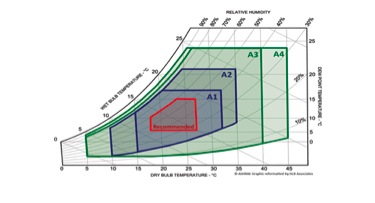
\includegraphics[width=5in]{fig2}
\caption{IT equipment environmental classes}
\label{fig:ITenviron}
\end{figure}


\label{sec:cooling}

\end{document}
